\documentclass[8pt,a4paper,compress]{beamer}

\usepackage{/home/siyer/lib/slides}

\title{Quick Sort}
\date{}

\begin{document}
\begin{frame}
\vfill
\titlepage
\end{frame}

\begin{frame}
\frametitle{Outline}
\tableofcontents
\end{frame}

\section{The Basic Algorithm}
\begin{frame}[fragile]
\begin{itemize}
\item quick sort is a divide-and-conquer method for sorting, and it  works by partitioning an array into two subarrays, then sorting the subarrays independently

\smallskip

\begin{center}
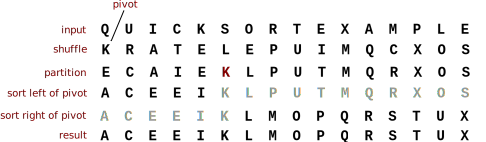
\includegraphics[scale=0.6]{{./figures/quicksort_overview}.pdf}
\end{center}
\end{itemize}
\end{frame}

\begin{frame}[fragile]
\begin{itemize}
\item the basic algorithm
\begin{lstlisting}[language=Java]
public class Quick {
    ...
    public static void sort(Comparable[] a) {
        StdRandom.shuffle(a);
        sort(a, 0, a.length - 1);
    }

    private static void sort(Comparable[] a, int lo, int hi) { 
        if (hi <= lo) { return; }
        int j = partition(a, lo, hi);
        sort(a, lo, j - 1);
        sort(a, j + 1, hi);
    }
    ...
}
\end{lstlisting}
\end{itemize}
\end{frame}

\begin{frame}[fragile]
\begin{itemize}
\item trace

\begin{center}
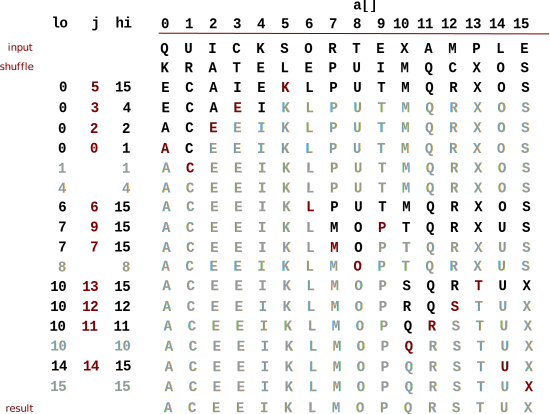
\includegraphics[scale=0.6]{{./figures/quicksort_trace}.pdf}

\smallskip

the basic quick sort algorithm
\end{center}
\end{itemize}
\end{frame}

\begin{frame}[fragile]
\begin{itemize}
\item the partitioning procedure rearranges the array such that
\begin{itemize}
\item the entry \lstinline{a[j]} is in its final place in the array, for some \lstinline{j}
\item no entry in \lstinline{a[lo]} through \lstinline{a[j - 1]} is greater than \lstinline{a[j]}
\item no entry in \lstinline{a[j + 1]} through \lstinline{a[hi]} is less than \lstinline{a[j]}
\end{itemize}

\begin{lstlisting}[language=Java]
    ...
    private static int partition(Comparable[] a, int lo, int hi) {
        int i = lo;
        int j = hi + 1;
        Comparable v = a[lo];
        while (true) { 
            while (less(a[++i], v)) { if (i == hi) { break; } }
            while (less(v, a[--j])) { if (j == lo) { break; } }
            if (i >= j) { break; }
            exch(a, i, j);
        }
        exch(a, lo, j);
        return j;
    }
    ...
\end{lstlisting}
\end{itemize}
\end{frame}

\begin{frame}[fragile]
\begin{itemize}
\item trace

\begin{center}
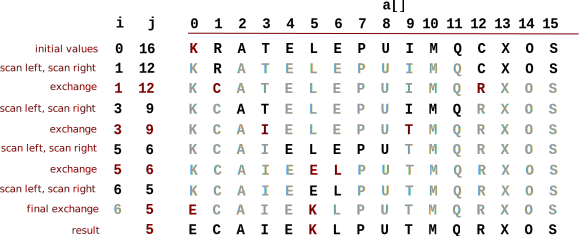
\includegraphics[scale=0.6]{{./figures/partition_trace}.pdf}

\smallskip

partitioning (array contents before and after each exchange)
\end{center}

\item quick sort uses $\sim 2N\ln N$ comparisons and $\sim N/3\ln N$ exchanges on the average to sort an array of length $N$ with distinct keys; and $\sim N^2/2$ comparisons in the worst case, but random shuffling protects against this case
\end{itemize}
\end{frame}

\section{Algorithmic Improvements}
\begin{frame}[fragile]
\begin{itemize}
\item an easy way to improve the performance of quick sort is to use insertion sort for tiny subarrays, ie, replace the following statement 
\begin{lstlisting}[language=Java]
if (hi <= lo) { return; }
\end{lstlisting}
in the recursive \lstinline{Quick.sort()} method with the following statement
\begin{lstlisting}[language=Java]
if (hi <= lo + M) { Insertion.sort(a, lo, hi); return; }
\end{lstlisting}
where the optimum value of the cutoff $M$ is system-dependent, but any value between 5 and 15 is likely to work well in most situations

\item a second easy way to improve the performance of quick sort is to use the median of a small sample of items (usually three) taken from the subarray as the partitioning item
\end{itemize}
\end{frame}

\begin{frame}[fragile]
\begin{itemize}
\item when arrays have a large number of duplicate keys (eg, sorting a large personnel file by year of birth), one straightforward idea (due to Dijkstra), called 3-way quick sort, is to partition the array into three parts, one each for items with keys smaller than, equal to, and larger than the partitioning item's key
\begin{lstlisting}[language=Java]
public class Quick3way {
    ...
    private static void sort(Comparable[] a, int lo, int hi) { 
        if (hi <= lo) return;
        int lt = lo, gt = hi;
        Comparable v = a[lo];
        int i = lo;
        while (i <= gt) {
            int cmp = a[i].compareTo(v);
            if      (cmp < 0) { exch(a, lt++, i++); }
            else if (cmp > 0) { exch(a, i, gt--); }
            else              { i++; }
        }
        sort(a, lo, lt - 1);
        sort(a, gt + 1, hi);
    }
    ...
}
\end{lstlisting}
\end{itemize}
\end{frame}

\begin{frame}[fragile]
\begin{itemize}
\item trace
\begin{center}
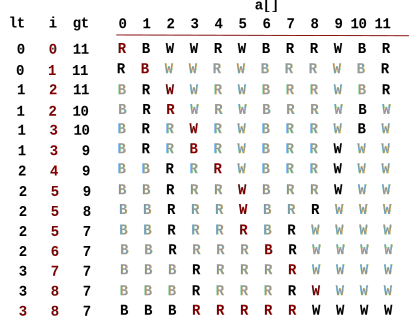
\includegraphics[scale=0.6]{{./figures/quick3way_trace}.pdf}

\smallskip

3-way quick sort (array contents after each iteration)
\end{center}
\end{itemize}
\end{frame}

\begin{frame}[fragile]
\begin{itemize}
\item given $N$ keys with $k$ distinct key values, for each $i$ from 1 to $k$ define $f_i$ to be frequency of occurrence of the $i$th key value and $p_i$  to be $f_i/N$, the probability that
the $i$th key value is found when a random entry of the array is sampled

\item the Shannon entropy of the keys (a classic measure of their information content) is defined as
\begin{eqnarray}
H &=& -(p_1\lg p_1 + p_2\lg p_2 + \dots + p_k\lg p_k) \nonumber \\
  &=& -\sum_{i=1}^k p_i\lg p_i \nonumber 
\end{eqnarray}

\item no comparison-based sorting algorithm can guarantee to sort $N$ items with fewer than $NH-N$ comparisons, where $H$ is the Shannon entropy, defined from the frequencies of key values


\item 3-way quick sort uses $\sim (2\ln 2)NH$ comparisons to sort $N$ items, where $H$ is the Shannon entropy, defined from the frequencies of key values
\end{itemize}
\end{frame}

\section{Quick Sort and Other Sorts}
\begin{frame}[fragile]
\begin{itemize}
\item a comparison of merge sort and other sorts seen so far
\begin{lstlisting}[language={}]
$ java SortCompare Quick Insertion 10000 100
For 10000 random Doubles
    Quick is 31.3 times faster than Insertion
\end{lstlisting}

\begin{lstlisting}[language={}]
$ java SortCompare Quick Shell 10000 100
For 10000 random Doubles
    Quick is 0.7 times faster than Shell
\end{lstlisting}

\begin{lstlisting}[language={}]
$ java SortCompare Quick Merge 10000 100
For 10000 random Doubles
    Quick is 1.1 times faster than Merge
\end{lstlisting}

\begin{lstlisting}[language={}]
$ java SortCompare Quick System 10000 100
For 10000 random Doubles
    Quick is 1.9 times faster than System
\end{lstlisting}
\end{itemize}
\end{frame}
\end{document}
